\chapter{Evaluation and Result Analysis}\label{ch:eval}

This chapter reports the Vermont benchmark comparison based on the selected
experiment set. The numerical statements below are based on the consolidated
outputs from
\texttt{summarize\_selected\_experiment\_metrics}, together with the exported
\texttt{results}, \texttt{wandb}, and \texttt{target\_folder} files.

中文：本章基于当前选定实验集的结果，报告当前的 Vermont 基准对比。下面的数值主要来自
\texttt{summarize\_selected\_experiment\_metrics} 的汇总表，以及
\texttt{results}、\texttt{wandb} 和 \texttt{target\_folder} 中导出的测试结果。

\section{Evaluation Scope}

The experiments use the Annex 96 Common Exercise 1 CityLearn portfolios. Each
portfolio contains 25 single-family homes with photovoltaic generation and
battery storage. The fully summarized comparison in this report is the Vermont
setting, where January is used for training and February is used for testing.
Texas remains future work for the RL comparison, so the conclusions in this
chapter should be read as Vermont benchmark conclusions rather than
cross-climate conclusions.

中文：实验使用 Annex 96 Common Exercise 1 的 CityLearn 建筑组合。每个组合包含
25 栋带光伏和电池的独立住宅。当前已经完整汇总的是 Vermont 场景，其中 1 月用于训练，
2 月用于测试。Texas 的 RL 对比仍然是后续工作，因此本章结论应理解为 Vermont
基准结论，而不是跨气候结论。

\begin{table}[h]
\begin{center}
\begin{tabular}{|l|l|l|l|}
\hline
Climate & Training month & Testing month & Current status \\
\hline
Vermont & January & February & fully summarized in this report \\
Texas & August & September & RL comparison remains future work \\
\hline
\end{tabular}
\end{center}
\caption{Annex 96 train/test split and current evaluation scope.}
\label{tab:split}
\end{table}

The selected Vermont comparison contains 15 representative runs: RBC,
independent PPO and SAC baselines, standard MAPPO, grouped MAPPO, and the main
communication variants. Under the current hardware constraints, most MAPPO
experiments in the selected set were trained for about 500 episodes and reached
rough convergence, although some communication methods such as TarMAC may still
improve further. The independent PPO and SAC results are also useful
references, but because these methods require more training time and higher
computational cost, in this report they are mainly used as important references
after the sum reward and each agent's reward had roughly converged.

中文：当前选定的 Vermont 对比一共包含 15 个代表性实验：RBC、独立 PPO 和 SAC、
标准 MAPPO、分组 MAPPO，以及主要通信变体。受当前硬件条件限制，多数 MAPPO 系列实验选取训练到
500 个 episode 左右并达到大致收敛。不过，部分通信方法，例如 TarMAC，仍然可能继续提升。
独立 PPO 和 SAC 的结果也有参考价值，但由于这两类方法训练时间更长、成本更高，本报告主要将它们训练到
sum reward和每个智能体的 reward 大致收敛后作为重要的参考。

\section{Overall Ranking Summary}

The ranking tables show that there is currently no method that is absolutely
best under every reading of the task. In the current Vermont result set,
\texttt{mappo\_grouped\_powernet\_global} ranks first in the
overall ranking. The secondary metrics are not explicitly included in the
reward function, but they are still useful as references, because they show
which methods already behave well on those objectives even without being
directly optimized. However, if the comparison is restricted to the primary
metrics, namely CV-RMSE, $|$NMBE$|$, and comfort, the top method becomes
\texttt{mappo\_grouped\_comm\_weighted\_default}.

中文：排序表说明，目前这个任务下并不存在一个在所有理解方式下都绝对最优的方法。
在当前 Vermont 结果集中，
\texttt{mappo\_grouped\_powernet\_global}
在综合总排名中排第一（次要指标还未计入reward function中，但是仍然可以作为参考，即在没有计入计算的情况下，哪种方法就已经在次要指标上表现上良好了）。
但如果只看主要指标，也就是 CV-RMSE、$|$NMBE$|$ 和舒适性，
排第一的是
\texttt{mappo\_grouped\_comm\_weighted\_default}。

\begin{table}[h]
\scriptsize
\begin{center}
\begin{tabular}{|l|r|r|r|r|r|}
\hline
Controller & Primary rank & Primary score & CV-RMSE (\%) & $|$NMBE$|$ (\%) & Comfort hours \\
\hline
Grouped MAPPO + Weighted Default & 1 & 3.33 & 48.68 & 2.31 & 3166 \\
Grouped MAPPO + PowerNet Global & 2 & 3.75 & 46.45 & 0.43 & 4359 \\
RLlib Independent PPO & 3 & 4.00 & 49.76 & 1.24 & 2309 \\
Grouped MAPPO + Weighted $(0.90,0.10)$ & 4 & 4.83 & 49.75 & 1.95 & 3308 \\
Grouped MAPPO + Weighted $(0.55,0.45)$ & 5 & 5.33 & 49.28 & 0.27 & 5376 \\
Grouped MAPPO & 6 & 6.92 & 51.50 & 2.75 & 3520 \\
Grouped MAPPO + TarMAC & 7 & 7.00 & 49.65 & 3.32 & 3713 \\
Grouped MAPPO + GAT & 8 & 7.75 & 51.35 & 2.92 & 3866 \\
Grouped MAPPO + CommNet & 9 & 8.75 & 48.94 & 8.11 & 4873 \\
RLlib SAC & 10 & 9.25 & 46.53 & 8.93 & 7470 \\
Grouped MAPPO + Comm v2 & 11 & 10.08 & 52.92 & 3.80 & 4031 \\
Standard MAPPO & 12 & 10.42 & 53.30 & 5.29 & 3542 \\
Grouped MAPPO + DIAL & 13 & 11.33 & 52.39 & 7.25 & 6755 \\
Grouped MAPPO + PowerNet & 14 & 12.42 & 50.16 & 9.15 & 7685 \\
RBC baseline & 15 & 14.83 & 138.27 & 109.37 & 11465 \\
\hline
\end{tabular}
\end{center}
\caption{Primary-only ranking for the selected Vermont experiments.}
\label{tab:vt-rank-summary}
\end{table}

The primary-only ranking gives a clearer picture of the main tracking objective.
The best primary-score balance now comes from the default weighted
communication setting, here the default weights are
\mbox{$\alpha=0.75,\beta=0.25$}. It combines low CV-RMSE, moderate bias, and a
strong comfort result. The PowerNet Global variant ranks second because it has the best
CV-RMSE and the smallest absolute NMBE in the main MAPPO set, but it gives up
more comfort than the weighted default controller. The independent PPO baseline
ranks third and has especially strong comfort performance, but its CV-RMSE and
absolute NMBE are weaker than the top two methods, likely because it does not
model explicit inter-building coordination and therefore cannot optimize the
portfolio-level tracking objective as directly as the grouped communication
methods.

中文：只看主要指标的排名，会更清楚地反映核心跟踪任务的表现。
当前主要指标上最均衡的方法是默认加权通信，这里默认权重是
\mbox{$\alpha=0.75,\beta=0.25$}，它同时给出了较低的 CV-RMSE、
适中的偏差，以及较好的舒适性结果。PowerNet Global 排第二，
因为它在主要 MAPPO 方法中给出了最好的 CV-RMSE 和最小的绝对 NMBE，
但它在舒适性上不如默认加权通信。独立 PPO 排第三，
并且在舒适性上尤其强，但它在 CV-RMSE 和绝对 NMBE 上不如前两者，
一个更直接的原因是它没有显式建模建筑之间的协同关系，因此不如前两种分组通信方法那样，
能够直接围绕组合层面的跟踪目标进行优化。

For completeness, Table~\ref{tab:vt-overall-composite} reports the overall
composite ranking generated by
\texttt{summarize\_selected\_experiment\_metrics}. Unlike the primary-only
table above, this ranking also reflects selected secondary objectives, so it is
useful for understanding why the final ``overall best'' method is not exactly
the same as the primary-only winner.

中文：为了完整起见，表~\ref{tab:vt-overall-composite} 给出了
\texttt{summarize\_selected\_experiment\_metrics} 生成的综合总排名。
和上面的主指标表不同，这个排名还会受到部分次级指标的影响，因此它可以帮助解释：
为什么最终的“综合最优”方法，并不完全等同于主指标排名第一的方法。

\begin{table}[h]
\scriptsize
\begin{center}
\begin{tabular}{|l|r|r|r|r|r|r|}
\hline
Controller & Overall rank & Overall score & Primary rank & Recommended rank & Peak change (\%) & Ramping (kW) \\
\hline
Grouped MAPPO + PowerNet Global & 1 & 5.14 & 2 & 3 & -4.19 & 478.22 \\
RLlib SAC & 2 & 5.60 & 10 & 7 & -18.80 & 353.48 \\
RLlib Independent PPO & 3 & 5.87 & 3 & 1 & -2.69 & 372.06 \\
Grouped MAPPO + TarMAC & 4 & 6.22 & 7 & 6 & -1.38 & 486.31 \\
Grouped MAPPO + Weighted Default & 5 & 6.48 & 1 & 2 & 5.13 & 429.05 \\
Grouped MAPPO + CommNet & 6 & 6.77 & 9 & 8 & -4.45 & 441.78 \\
Grouped MAPPO + Weighted $(0.90,0.10)$ & 7 & 6.98 & 4 & 4 & -2.20 & 443.12 \\
Grouped MAPPO + Weighted $(0.55,0.45)$ & 8 & 8.15 & 5 & 5 & 0.54 & 463.45 \\
Grouped MAPPO & 9 & 8.19 & 6 & 9 & -1.19 & 519.14 \\
Grouped MAPPO + Comm v2 & 10 & 9.03 & 11 & 12 & -0.05 & 498.03 \\
Grouped MAPPO + DIAL & 11 & 9.19 & 13 & 11 & -2.04 & 498.95 \\
Grouped MAPPO + GAT & 12 & 9.29 & 8 & 10 & -0.15 & 537.38 \\
Grouped MAPPO + PowerNet & 13 & 9.64 & 14 & 14 & -0.63 & 459.18 \\
Standard MAPPO & 14 & 10.40 & 12 & 13 & 9.28 & 506.42 \\
RBC baseline & 15 & 13.06 & 15 & 15 & -8.44 & -- \\
\hline
\end{tabular}
\end{center}
\caption{Overall composite ranking for the selected Vermont experiments.}
\label{tab:vt-overall-composite}
\end{table}

\section{Primary and Secondary Metric Overview}

The primary objective is portfolio-level reference tracking. Let $y_t$ be the
actual aggregate portfolio load and $r_t$ be the reference load. The two main
tracking metrics are NMBE and CV-RMSE:

中文：首要目标仍然是建筑组合层面的负荷跟踪。记 $y_t$ 为实际组合负荷，
$r_t$ 为参考负荷。核心跟踪指标仍然是 NMBE 和 CV-RMSE：
\begin{equation}
\mathrm{NMBE} =
\frac{\frac{1}{T}\sum_{t=1}^{T}(y_t-r_t)}
{\frac{1}{T}\sum_{t=1}^{T}r_t} \times 100\%,
\end{equation}

\begin{equation}
\mathrm{CV\mbox{-}RMSE} =
\frac{\sqrt{\frac{1}{T}\sum_{t=1}^{T}(y_t-r_t)^2}}
{\frac{1}{T}\sum_{t=1}^{T}r_t} \times 100\%.
\end{equation}

Lower absolute NMBE and lower CV-RMSE mean better tracking. At the same time,
comfort exceedance hours, here mainly temperatures above
\(24^\circ\mathrm{C}\) or below \(20^\circ\mathrm{C}\), must also be reported,
because a controller that tracks the target well but causes many temperature
violations is still not a good practical solution.

中文：$|$NMBE$|$ 越低、CV-RMSE 越低，说明跟踪越好。与此同时，还必须同时看
舒适性超限小时数（在这里是超过24或者低于20），因为如果一个控制器虽然跟踪好了目标，但造成大量温度越界，
它在实际中仍然不算好方案。

\begin{figure}[h]
\begin{center}

\includegraphics[width=0.92\textwidth]{figures/selected_experiment_primary_metrics.png}
\end{center}
\caption{Primary metric summary for the selected Vermont experiments.}
\label{fig:primary-summary}
\end{figure}

\begin{figure}[h]
\begin{center}

\includegraphics[width=0.92\textwidth]{figures/selected_experiment_secondary_metrics.png}
\end{center}
\caption{Secondary metric summary for the selected Vermont experiments.}
\label{fig:secondary-summary}
\end{figure}

Figures~\ref{fig:primary-summary} and~\ref{fig:secondary-summary} show the main
trade-offs in the current results very clearly. The lowest CV-RMSE now comes
from PowerNet Global and SAC, but SAC is clearly worse in comfort and NMBE. The
weighted default communication run is not first overall, but it is the most
balanced method on the primary metrics because it combines a low CV-RMSE with
the fewest comfort-exceedance hours among the main MAPPO communication methods.
PowerNet Global ranks first overall because, even without secondary metrics
being trained explicitly, it has no obvious weakness across several categories:
it is second on the primary table, fourth on peak reduction, and sixth on
fairness.

中文：图~\ref{fig:primary-summary} 和图~\ref{fig:secondary-summary}
把当前结果中的主要取舍展示得很清楚。现在最低的 CV-RMSE 来自 PowerNet Global
和 SAC，但 SAC 的舒适性和 NMBE 明显更差。默认加权通信虽然不是综合第一，
但它在主要指标上表现最均衡，因为它同时给出了较低的 CV-RMSE，以及主要 MAPPO
通信方法里最少的舒适性超限小时数。PowerNet Global 能排综合第一，
是因为它在次要指标无训练的情况下，多个类别上都没有明显短板：主指标排第二，峰值削减排第四，公平性排第六。

\section{Best Run Diagnostics}

Because the overall best controller in this result set is
\texttt{mappo\_grouped\_powernet\_global}, it is useful to
look at its exported plots directly.

中文：由于当前新的综合最优实验是
\texttt{mappo\_grouped\_powernet\_global}，
下面直接看它导出的图，更容易理解这个结果为什么能排第一。

\begin{figure}[h]
\begin{center}
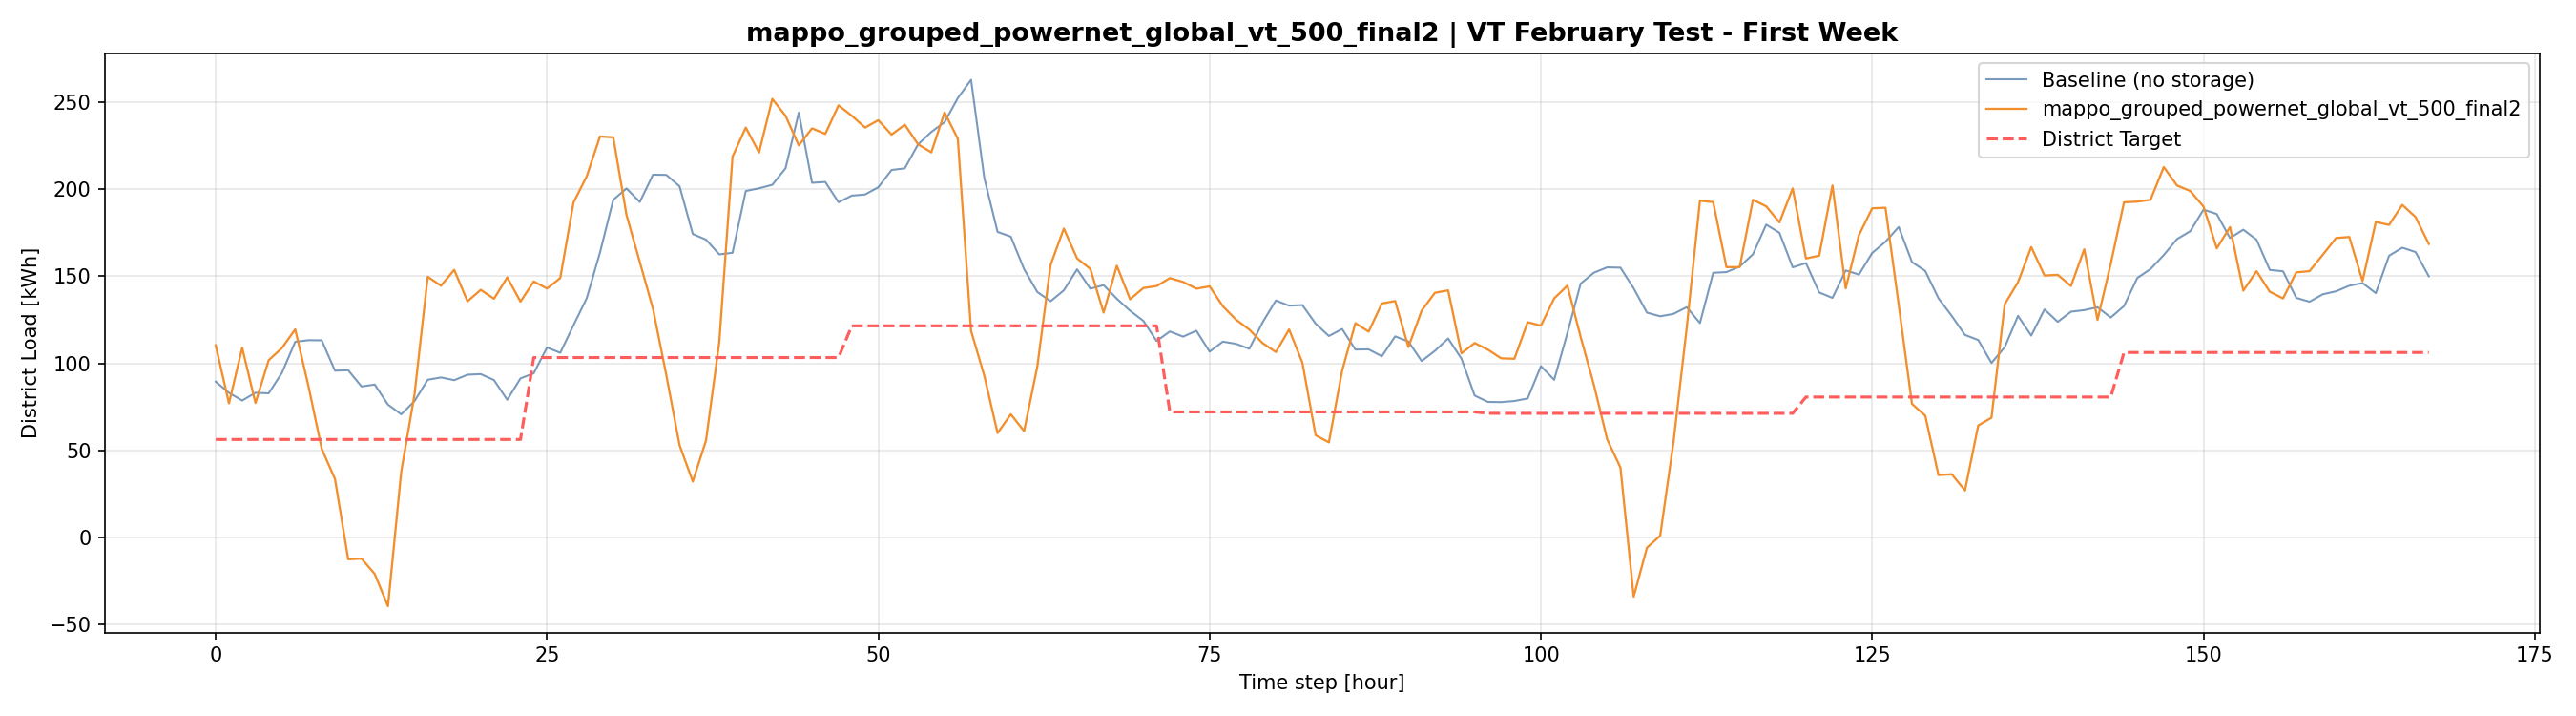
\includegraphics[width=0.92\textwidth]{figures/test_load_tracking_week1.png}
\end{center}
\caption{Week-1 aggregate load tracking for the best overall Vermont run.}
\label{fig:best-week1}
\end{figure}

\begin{figure}[h]
\begin{center}
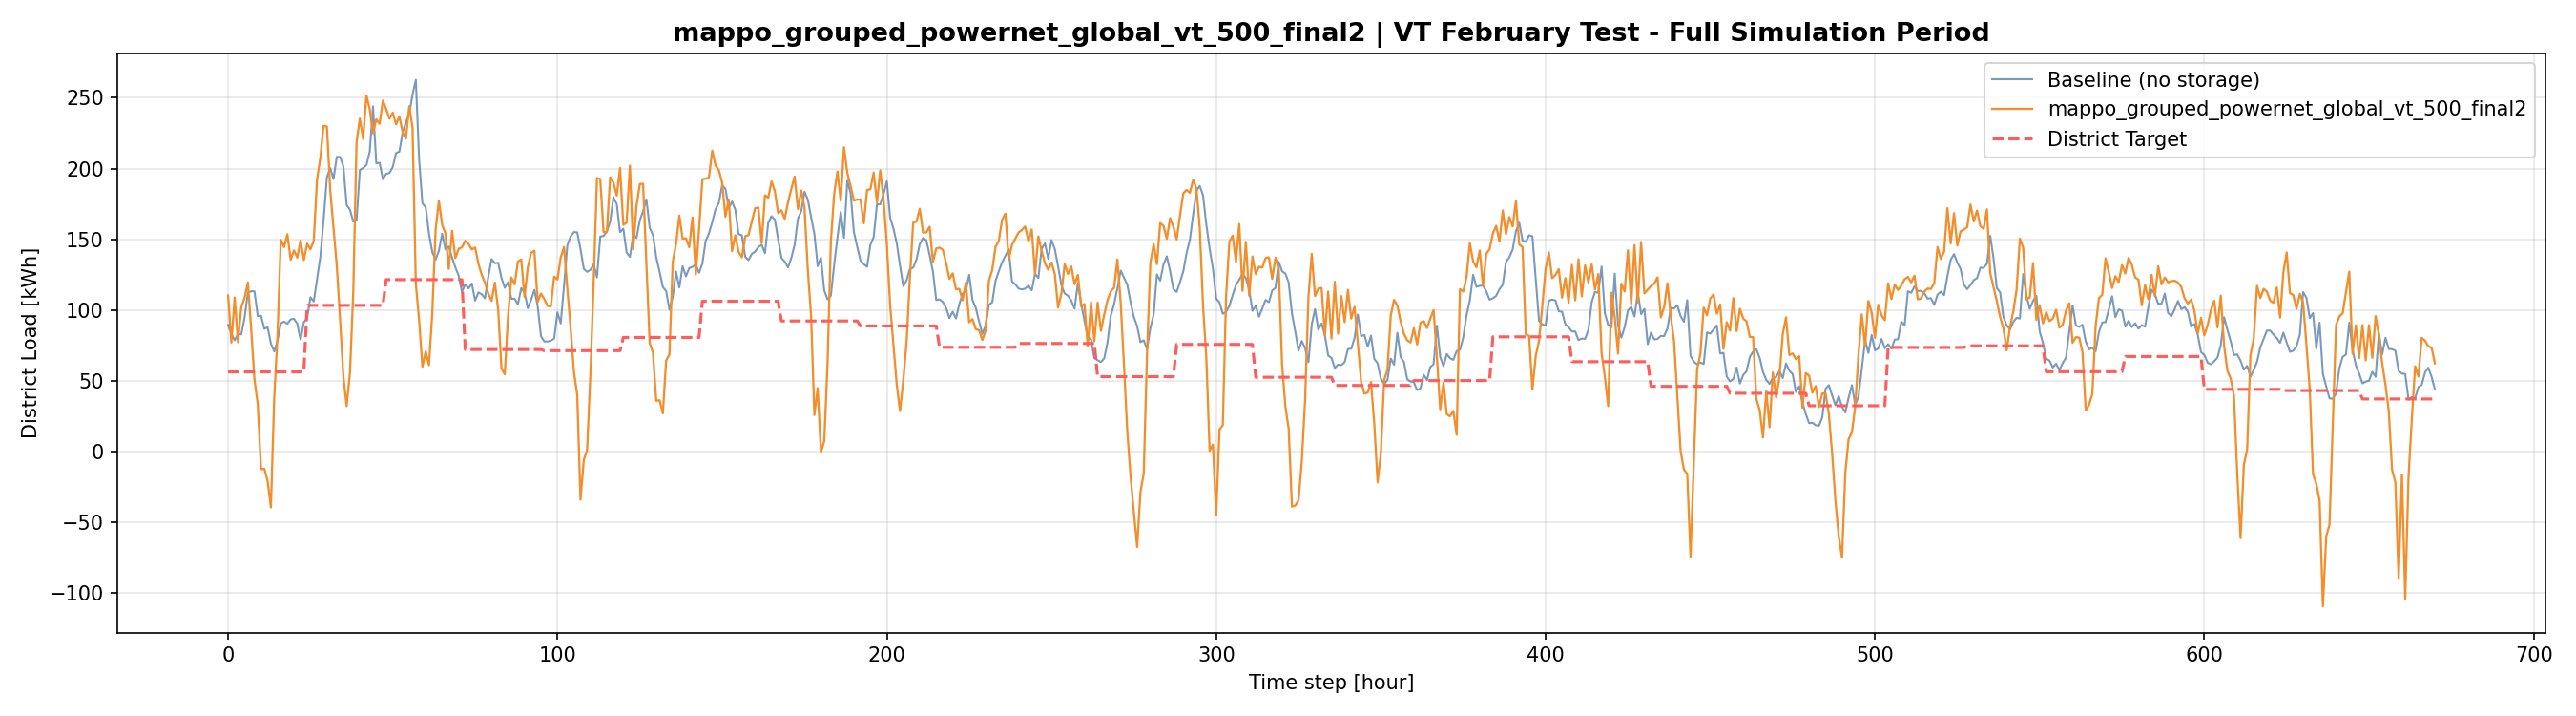
\includegraphics[width=0.92\textwidth]{figures/test_load_tracking_full.png}
\end{center}
\caption{Full-month aggregate load tracking for the best overall Vermont run.}
\label{fig:best-full}
\end{figure}

Figures~\ref{fig:best-week1} and~\ref{fig:best-full} show why this controller
is strong but not perfect. It reacts more aggressively than the no-storage
baseline and is able to shift the aggregate profile away from some high-load
periods, which helps the final CV-RMSE and peak-demand reduction. At the same
time, the response is sometimes too aggressive: the full-month plot contains
several deep downward excursions, including negative net-load periods. This is
consistent with the secondary metrics, where the same run is good on peak
demand but weak on ramping and peak-to-valley ratio.

中文：图~\ref{fig:best-week1} 和图~\ref{fig:best-full}
说明了这个控制器为什么强，但也不是没有代价。和无储能基线相比，
它的动作更积极，能够在一些高负荷时段把组合负荷移开，因此带来了更好的 CV-RMSE
和峰值削减。但它有时也会过于激进：整月图里可以看到多次很深的向下波动，
甚至出现负净负荷时段。这和次级指标是一致的，也就是它在峰值上表现不错，
但在爬坡和峰谷比上并不占优。

\begin{figure}[h]
\begin{center}
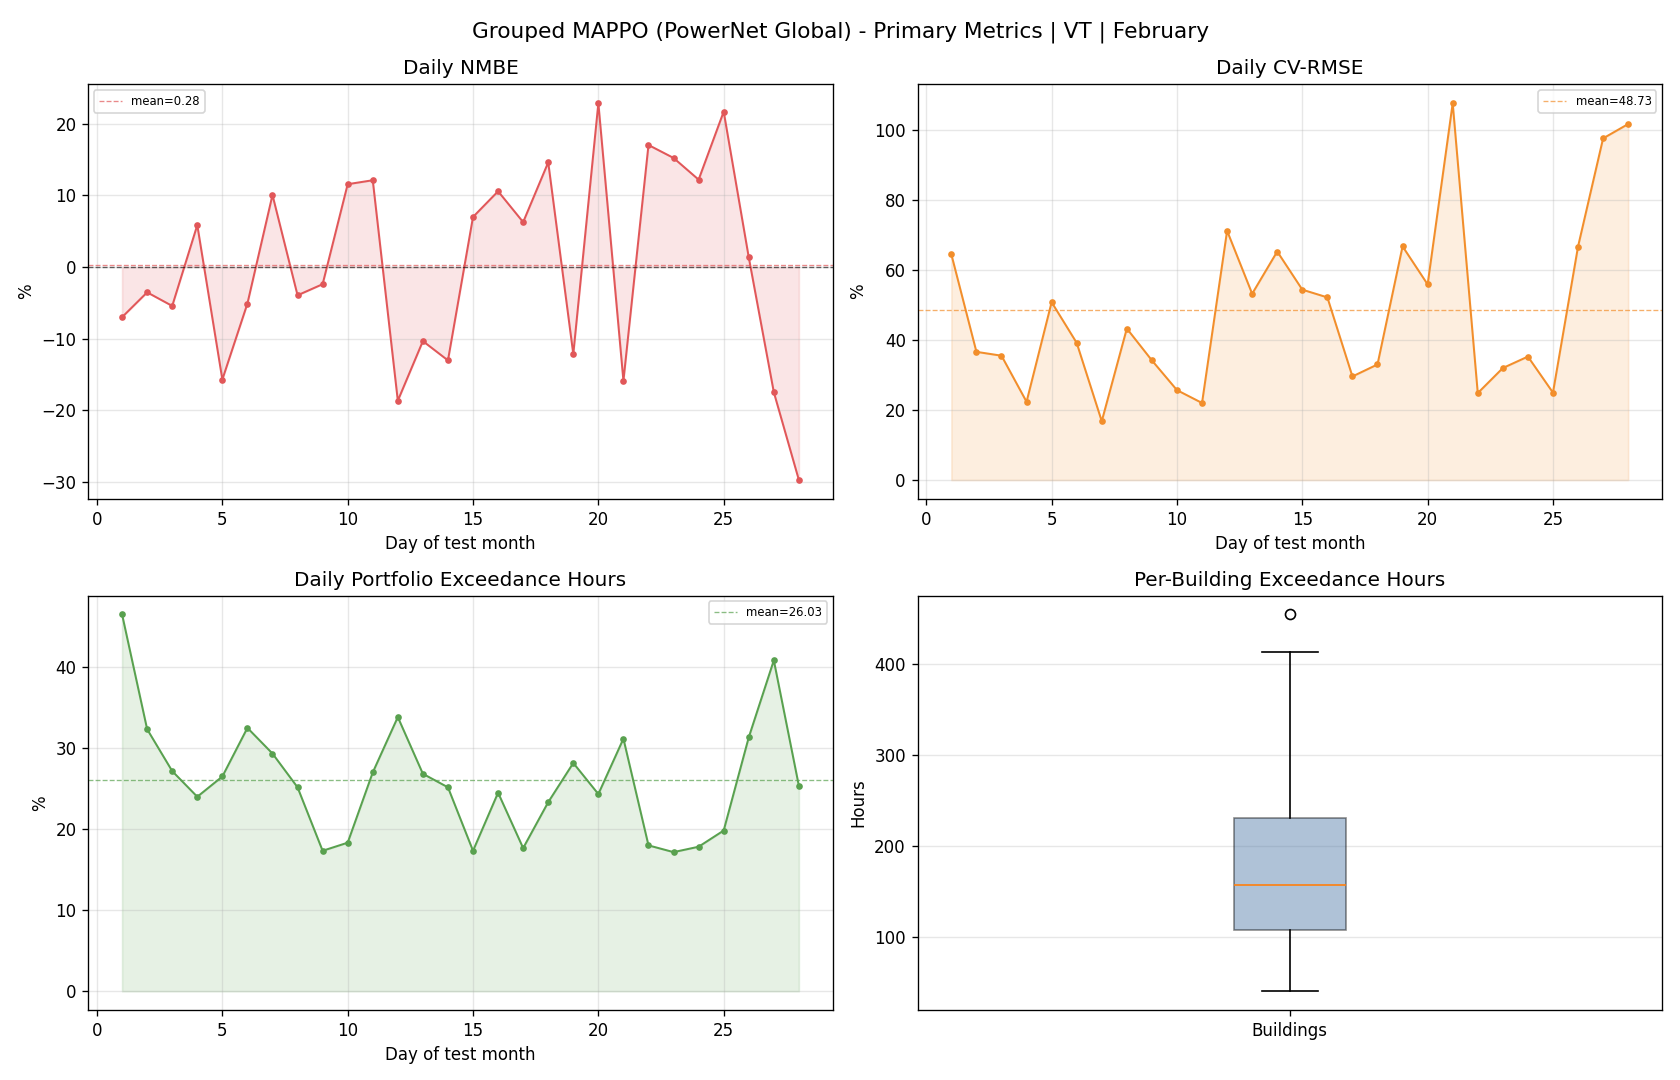
\includegraphics[width=0.92\textwidth]{figures/test_daily_metrics.png}
\end{center}
\caption{Daily primary metrics for the best overall Vermont run.}
\label{fig:best-daily}
\end{figure}

The daily metric plot gives the same conclusion in a more stable form. For the
best overall run, the daily NMBE mean is already close to zero, the daily
CV-RMSE mean is about 48.7\%, and the daily portfolio comfort exceedance mean
is about 26.0\%. However, the day-to-day variation is still quite large, and
some days are clearly better than others. The per-building comfort boxplot also
shows a wide spread: a few buildings contribute a large share of the total
violation hours. In this run, the worst building reaches about 454 exceedance
hours, compared with a mean of about 174.9 hours, which is roughly 2.6 times
the average, or about 160\% higher.

中文：日指标图给出了同样的结论，只是表达得更稳定一些。对这个综合最优实验来说，
日均 NMBE 已经很接近 0，日均 CV-RMSE 约为 48.7\%，组合层面的日均舒适性超限比例
约为 26.0\%。但它的逐日波动仍然比较大，有些天明显比其他天更好。
右下角的建筑舒适性箱线图也说明，超限小时数在不同建筑之间差异很大，
少数建筑贡献了较多的总超限小时（最差建筑约为 454 小时，平均约为 174.9 小时，
大约是平均值的 2.6 倍，或者说高出约 160\%）。

\begin{figure}[h]
\begin{center}
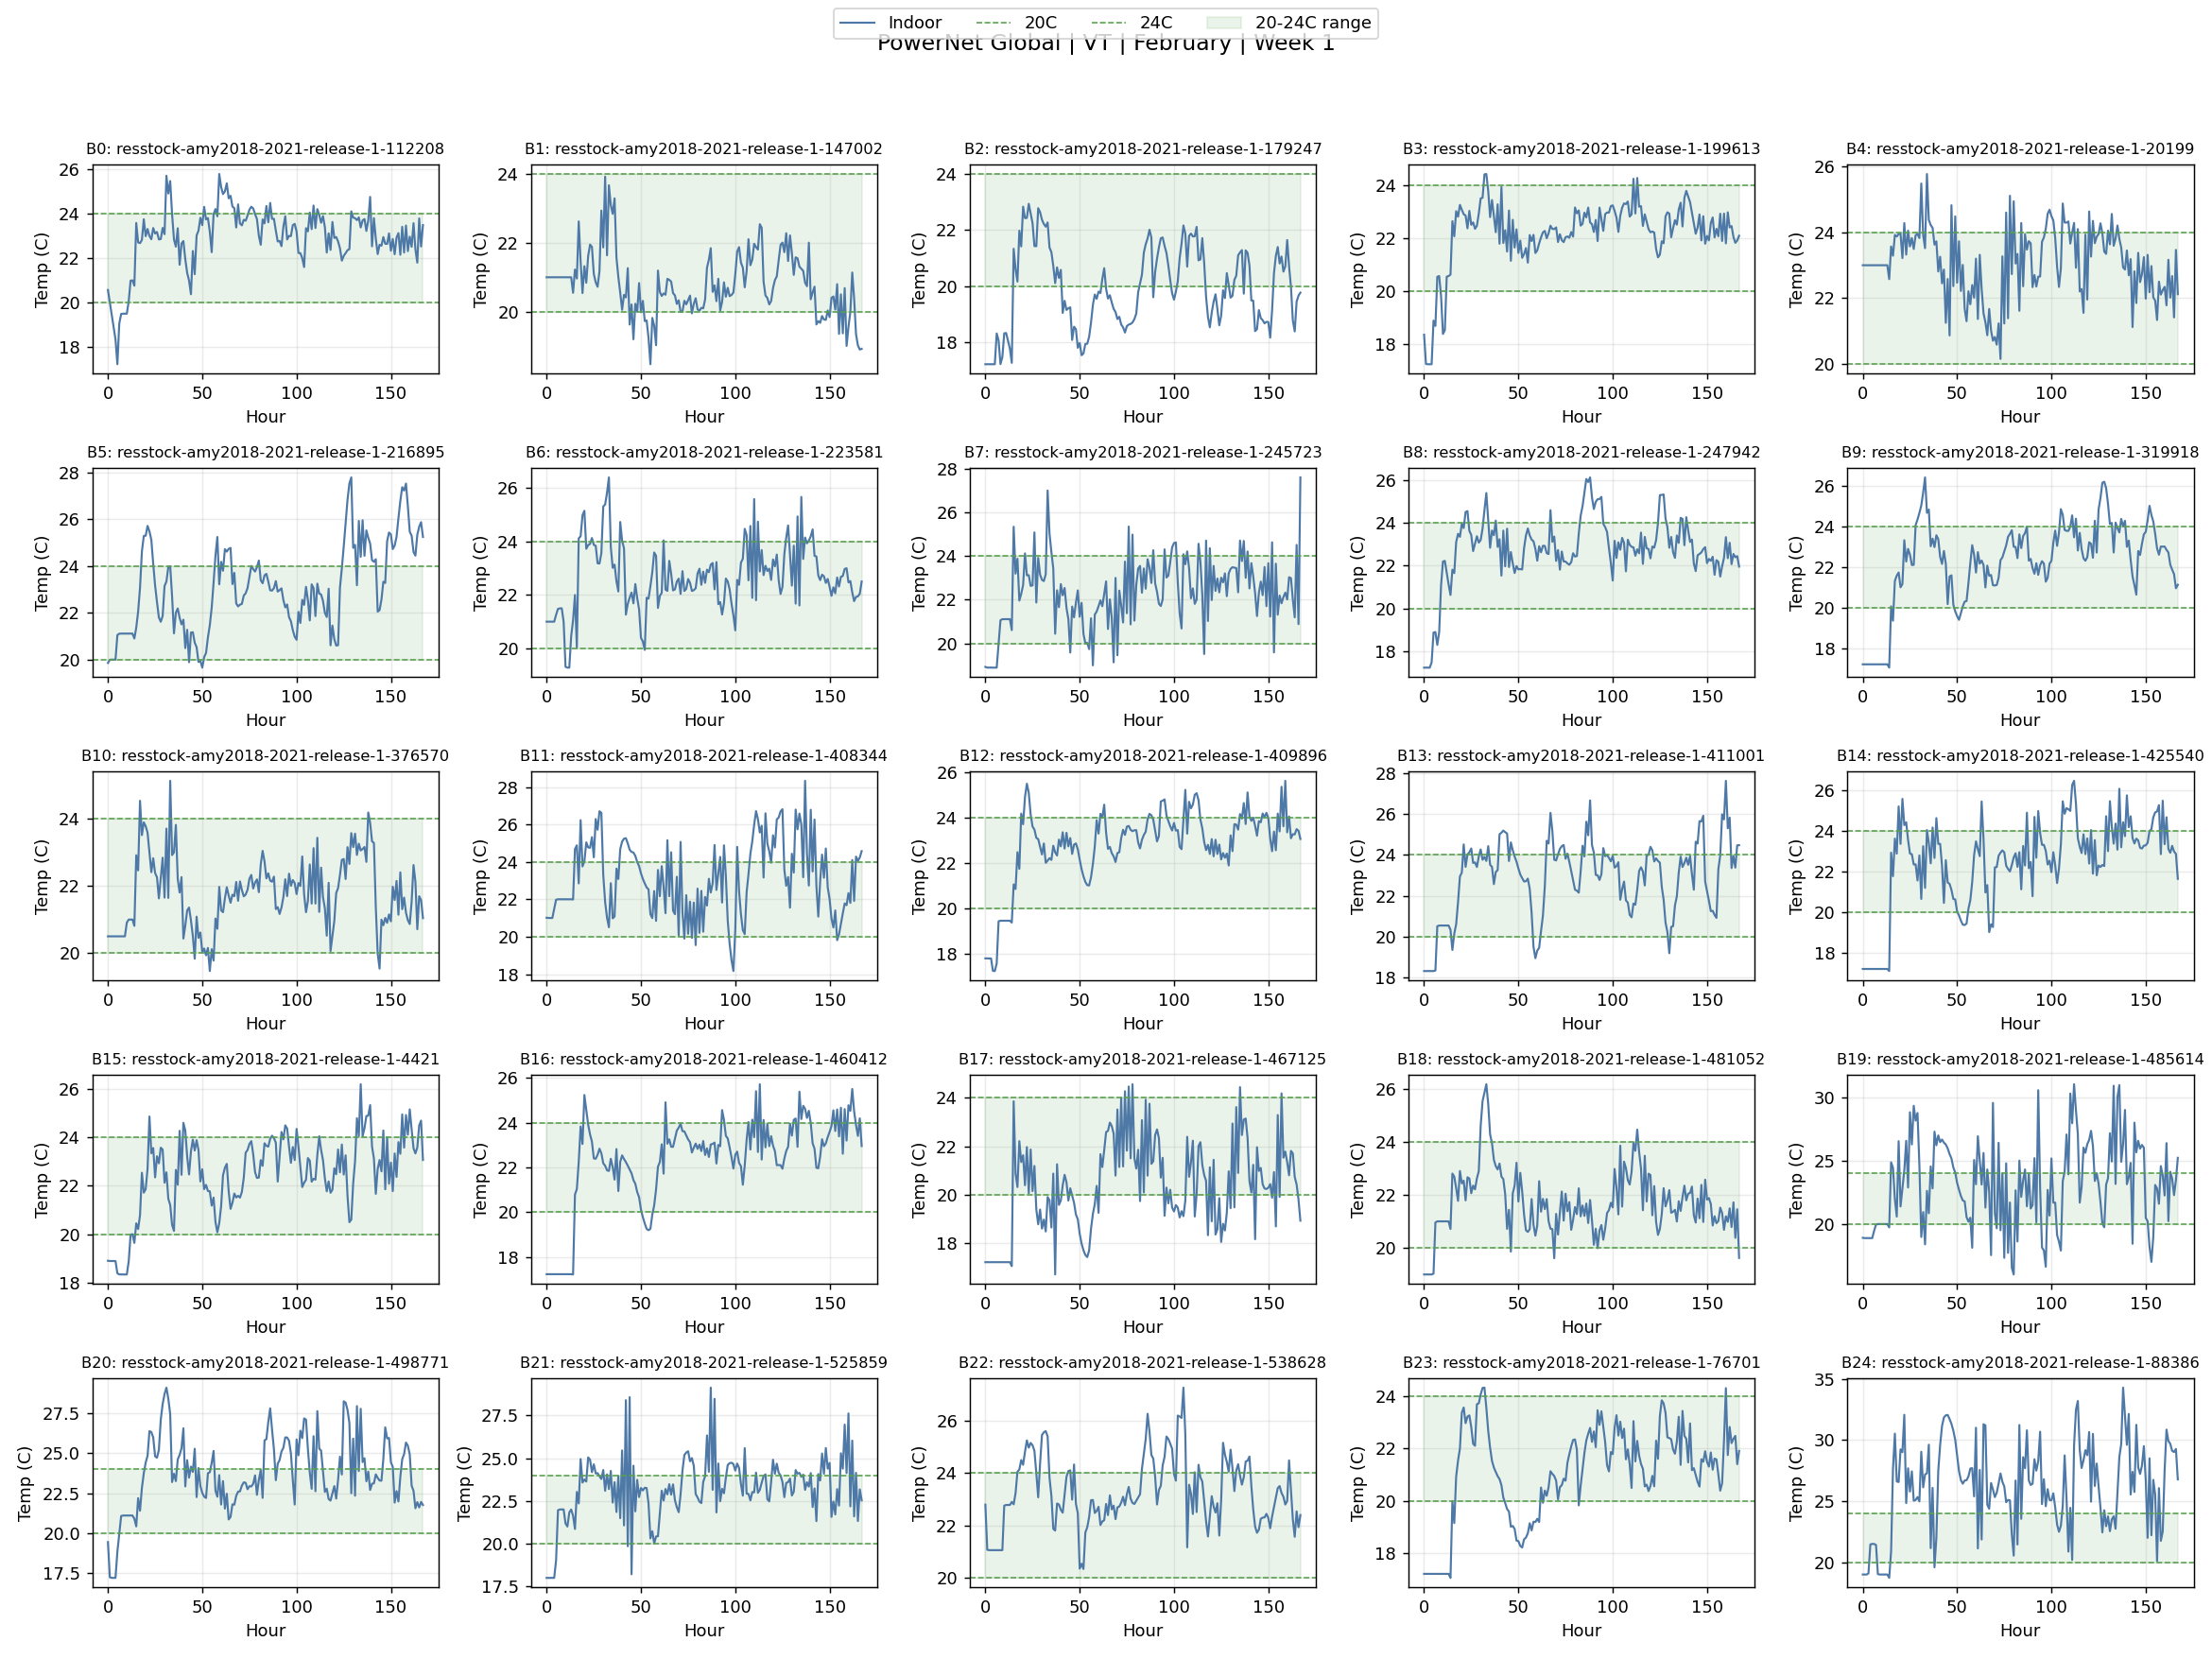
\includegraphics[width=0.92\textwidth]{figures/test_building_temperatures_week1.png}
\end{center}
\caption{Week-1 building temperature traces for the best overall Vermont run.}
\label{fig:best-temp-week1}
\end{figure}

\begin{figure}[h]
\begin{center}
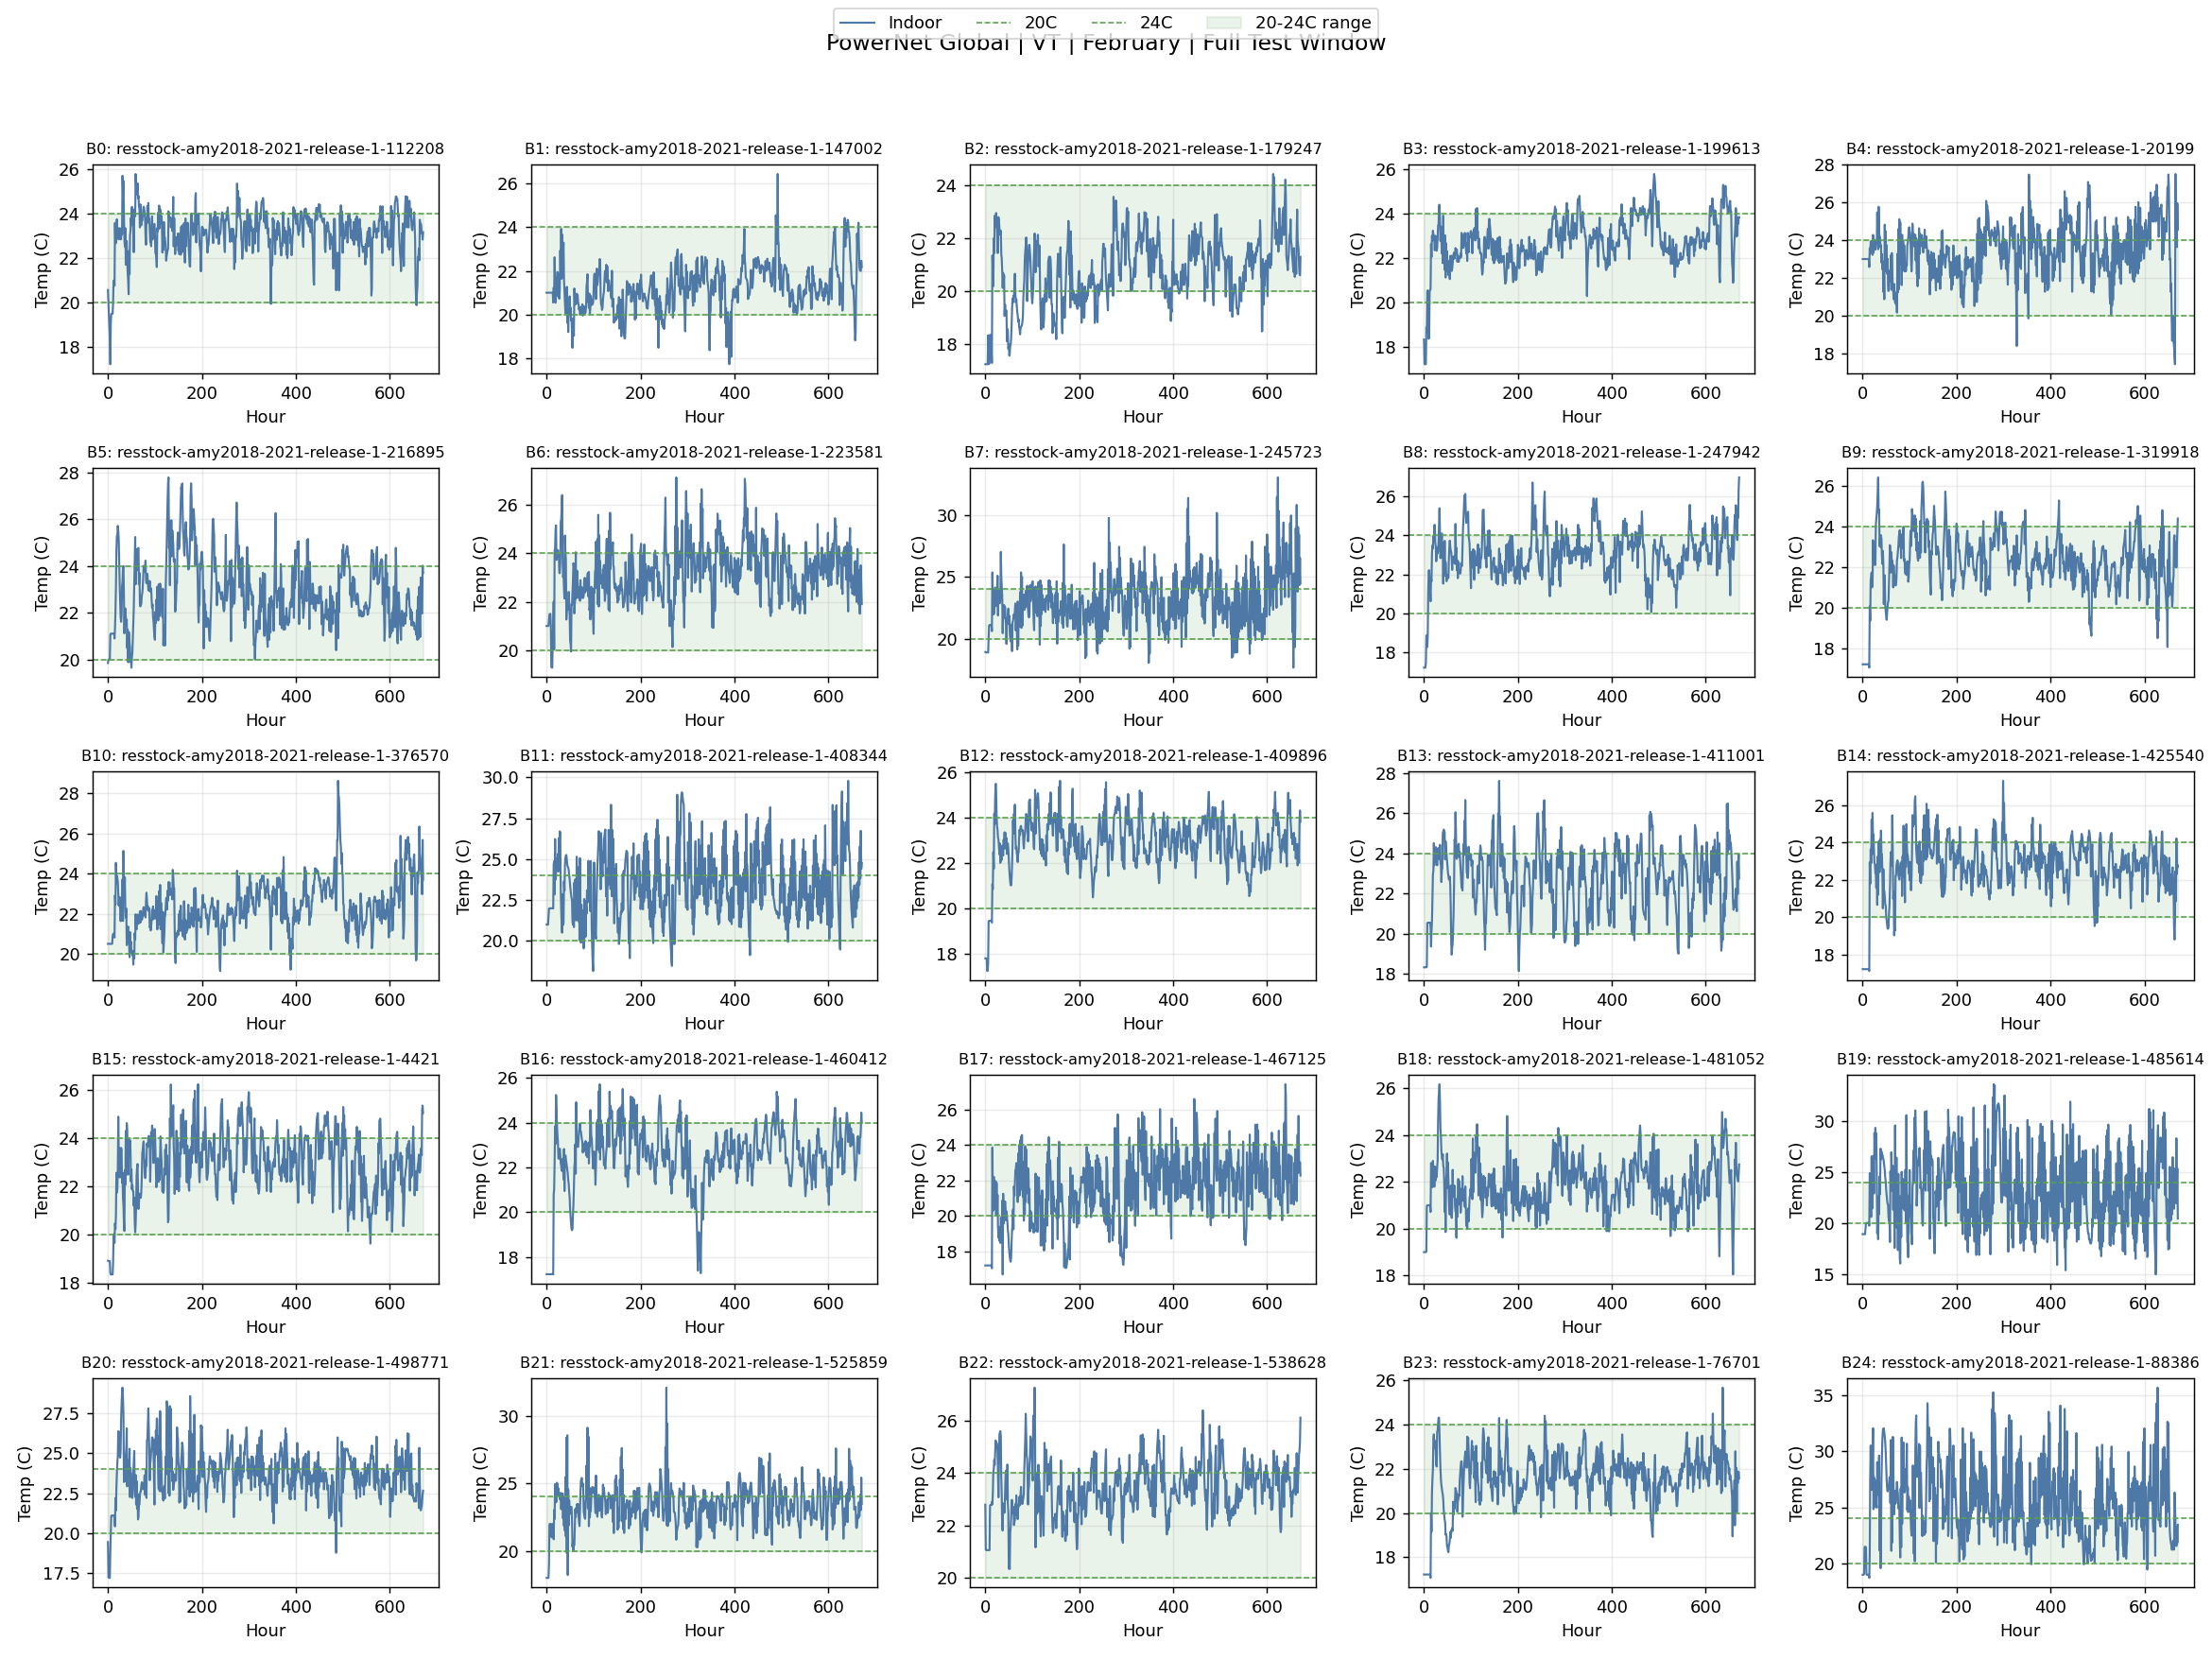
\includegraphics[width=0.92\textwidth]{figures/test_building_temperatures_full.png}
\end{center}
\caption{Full-month building temperature traces for the best overall Vermont run.}
\label{fig:best-temp-full}
\end{figure}

The temperature plots show that comfort is still the hardest part of the task.
Several homes stay near the comfort band for most of the month, but some homes
spend long periods above the upper bound. This is exactly why the best overall
controller is not the best comfort controller. In the exported comfort table,
the worst individual buildings still exceed 400 hours, while the easiest
buildings stay below 100 hours.

中文：温度图说明，舒适性仍然是这个任务里最难完全处理好的部分。一些住宅大部分时间
都维持在舒适区附近，但也有一些住宅会长时间高于上边界。这正是为什么综合第一的控制器，
并不是舒适性最优的控制器。从导出的舒适性表看，最差的建筑超限时间仍然超过 400 小时，
而最好的建筑则低于 100 小时。

\section{Communication Variant Comparison}

Table~\ref{tab:vt-comm-results} focuses only on the grouped communication
variants.

中文：表~\ref{tab:vt-comm-results} 只聚焦在分组通信变体上。

\begin{table}[h]
\scriptsize
\begin{center}
\begin{tabular}{|l|r|r|r|r|r|r|}
\hline
Method & Overall & Primary & Recommended & CV-RMSE (\%) & Comfort hours & Peak change (\%) \\
\hline
PowerNet Global & 1 & 2 & 3 & 46.45 & 4359 & -4.19 \\
TarMAC & 4 & 7 & 6 & 49.65 & 3713 & -1.38 \\
Weighted default & 5 & 1 & 2 & 48.68 & 3166 & 5.13 \\
CommNet & 6 & 9 & 8 & 48.94 & 4873 & -4.45 \\
Weighted $(0.90,0.10)$ & 7 & 4 & 4 & 49.75 & 3308 & -2.20 \\
Weighted $(0.55,0.45)$ & 8 & 5 & 5 & 49.28 & 5376 & 0.54 \\
Comm v2 & 10 & 11 & 12 & 52.92 & 4031 & -0.05 \\
DIAL & 11 & 13 & 11 & 52.39 & 6755 & -2.04 \\
GAT & 12 & 8 & 10 & 51.35 & 3866 & -0.15 \\
PowerNet & 13 & 14 & 14 & 50.16 & 7685 & -0.63 \\
\hline
\end{tabular}
\end{center}
\caption{Vermont comparison for grouped communication variants.}
\label{tab:vt-comm-results}
\end{table}

Based on the current results, several communication conclusions can be stated
more clearly. First, the strongest overall communication variant is
PowerNet Global. One direct interpretation is that when the PowerNet-style
block adds structured information from other agents, it first retains local
features; this can be understood as a form of information filtering or
cropping, so useful information is less likely to be overwritten during
communication \cite{powernet2020}. Second, the weighted communication family
shows that the weight setting itself has a clear effect on the final result.
Information from other groups can sometimes act as noise, but it can also
contain important portfolio-level information, so changing the same-group and
other-group weights changes the result substantially. Third, TarMAC can be seen
as an upgraded version of weighted communication: instead of using fixed
weights, it uses attention to let each agent learn which other buildings matter
more in the current state \cite{tarmac2019}. However, in the current
implementation, the underlying communication in TarMAC is still closer to
CommNet-style mean aggregation and does not yet incorporate the more selective
PowerNet-style structured information filtering or cropping
\cite{commnet2016}. This is why combining TarMAC with PowerNet remains a
promising direction. Finally, DIAL was originally proposed mainly for
DQN-style discrete-action settings. Its core idea is that differentiable
messages let agents see the feedback produced by their own communication
choices; during training, continuous messages are used to pass gradients, and
at execution time a sigmoid-like mechanism is used to approximate discrete
messages \cite{dial2016}. In the current MAPPO-based continuous-control
setting, this adapted DIAL performs poorly, which suggests that the original
DIAL idea does not transfer directly here.

中文：基于当前结果，可以更明确地给出几条通信结论。第一，当前综合最强的通信变体
是 PowerNet Global。一个比较直接的解释是，PowerNet 风格模块在加入结构化的其他智能体信息时，
会先保留本地特征，这本质上可以理解为一种信息裁剪方式，因此更不容易在通信过程中把原本有效的信息覆盖掉 \cite{powernet2020}。
第二，加权通信家族说明，权重设置本身就会明显影响结果。来自其他组的信息有时可能是噪声，
但也可能包含整个建筑组合层面的关键信息，因此组内和组外权重一变，最后结果就会明显变化。
第三，TarMAC 可以看成加权通信的升级版：它不再使用固定权重，而是通过 attention 机制让智能体自己学习，
当前状态下哪些建筑对自己更重要 \cite{tarmac2019}。不过在当前实现里，TarMAC 使用的底层通信仍然更接近
CommNet 风格的均值聚合，而没有结合 PowerNet 那种更有选择性的结构化信息裁剪方式 \cite{commnet2016}。
这也是为什么后续把 TarMAC 和 PowerNet 融合起来，仍然是一个很有希望的优化方向。最后，DIAL 原本主要是为
DQN 这类离散动作场景提出的，它的核心想法是让智能体通过可微消息看到自己通信选择带来的反馈；训练时先用连续消息传递梯度，
执行时再通过类似 sigmoid 的机制逼近离散消息 \cite{dial2016}。但在当前基于 MAPPO 的连续控制设置里，
这种改造后的 DIAL 效果并不好，这说明原始 DIAL 思路并不能直接平移到这里。

This communication table also shows why it is necessary to distinguish
``overall best,'' ``best comfort,'' and ``best primary score.'' In the current
setting, the secondary metrics are not explicitly included in the reward
function. The weighted default controller gives the best primary score and the
fewest comfort exceedance hours in Table~\ref{tab:vt-comm-results}, but it also
pushes peak demand above the baseline. This means that the secondary-metric
differences seen here are more natural results brought out by different
communication structures. PowerNet Global is not the best in comfort, but it is
more balanced across the primary objective and some secondary metrics, so it
ultimately ranks first overall. This also gives a useful direction for future
work that may explicitly include secondary metrics in the training objective.

中文：这张通信表也说明，必须区分“综合最优”“舒适性最优”和“主要指标最优”。
在当前 reward function 没有显式加入次要指标的情况下，
默认加权通信虽然在表~\ref{tab:vt-comm-results} 里给出了最好的主要指标得分，
舒适性超限也最少，但它反而让峰值负荷高于基线。这说明当前看到的次要指标差异，
更多是不同通信结构自然带出来的结果。PowerNet Global 的舒适性不是最好，
但它在主指标和部分次要指标之间更均衡，所以最终排到综合第一。
这也为后续把次要指标进一步纳入训练目标提供了一个很好的方向。

\section{Weighted Communication Ablation}

The weighted communication family is still valuable because it studies several
very specific questions on their own: how same-group and other-group messages
should be weighted, and whether it is necessary to let the agents learn those
weights themselves through attention.

中文：加权通信家族仍然很有研究价值，因为它单独研究了几个很具体的问题：
组内消息和组外消息到底应该如何分配权重，以及有没必要让只能体自己学会如何分配权重（也就是tarMAC的 attention 机制）

\begin{table}[h]
\scriptsize
\begin{center}
\begin{tabular}{|l|r|r|r|r|r|}
\hline
Weighted setting & Overall & Primary & CV-RMSE (\%) & Comfort hours & Peak change (\%) \\
\hline
Default $(0.75,0.25)$ & 5 & 1 & 48.68 & 3166 & 5.13 \\
$(0.90,0.10)$ & 7 & 4 & 49.75 & 3308 & -2.20 \\
$(0.55,0.45)$ & 8 & 5 & 49.28 & 5376 & 0.54 \\
\hline
\end{tabular}
\end{center}
\caption{Updated weighted communication ablation for Vermont.}
\label{tab:weighted-ablation}
\end{table}

This ablation shows that the simple claim ``putting more weight on same-group
information is always better'' is wrong. The exported results suggest that only
under specific weights does communication work best, and only then does
information from other groups stop acting like noise and start acting like a
gain. The default-weight setting \mbox{$\alpha=0.75,\beta=0.25$} is the
strongest on the primary metrics and also has the fewest comfort exceedance
hours. The \mbox{$(0.90,0.10)$} setting is slightly weaker on the pure primary
metrics, but it is more balanced. The more even \mbox{$(0.55,0.45)$} setting
almost removes NMBE bias, but its comfort result becomes clearly worse.

中文：这组消融结果可以看出“更强调组内信息就一定更好”这个简单说法是错误的。
导出结果说明，只有在特定的权重下，通讯效果才会最好，来自其他组的信息才不会是一种噪声，而是一种增益。
默认权重\mbox{$\alpha=0.75,\beta=0.25$} 设置在主要指标上最强，舒适性超限也最少。
\mbox{$(0.90,0.10)$} 在纯主要指标上略弱一点，
但更均衡；而更平均的 \mbox{$(0.55,0.45)$}
几乎消除了 NMBE 偏差，但舒适性明显变差。

\section{Rule-Based Baseline}

Table~\ref{tab:rbc-baseline-results} reports the available RBC notebook
comparison for Texas and Vermont. The RBC baseline is still useful as a
non-learning reference, but it is clearly much weaker than the learned
controllers on the CE1 load-tracking task.

中文：表~\ref{tab:rbc-baseline-results} 给出 notebook 中可用的 Texas 和
Vermont RBC 对比。RBC 仍然可以作为非学习型参考，但在 CE1 负荷跟踪任务上，
它明显弱于当前的学习型控制器。

\begin{table}[h]
\small
\begin{center}
\begin{tabular}{|l|r|r|r|r|}
\hline
Climate & NMBE RBC (\%) & NMBE baseline (\%) & CV-RMSE RBC (\%) & CV-RMSE baseline (\%) \\
\hline
TX & 89.57 & 79.12 & 207.63 & 163.74 \\
VT & 103.93 & 101.11 & 129.09 & 144.56 \\
\hline
\end{tabular}
\end{center}
\caption{RBC notebook baseline comparison against the CE1 target profile.}
\label{tab:rbc-baseline-results}
\end{table}

The RBC results still support the same broad conclusion: fixed hour-based
charge/discharge rules are not enough for the CE1 objective. In Vermont, RBC
improves CV-RMSE relative to the no-control baseline, but its bias remains
extremely large. In Texas, it is worse than the baseline on both NMBE and
CV-RMSE.

中文：RBC 的结论是：固定时段充放电规则不足以完成 CE1 的目标。
在 Vermont 中，RBC 虽然相对无控制基线改善了 CV-RMSE，但系统性偏差仍然很大；
在 Texas 中，它在 NMBE 和 CV-RMSE 上都比基线更差。

\section{Current Interpretation and Remaining Limits}

The Vermont results support four main conclusions. First, MARL is helpful for
this task. The stronger grouped MAPPO variants clearly outperform RBC, and
compared with independently trained PPO and SAC they also better show the
advantage of portfolio-level cooperative control; in particular, they avoid the
larger comfort cost seen in SAC and also make up for the lack of explicit
coordination in independent PPO. Second, communication clearly matters, but
there is no fixed answer to which communication method is best. In the current
results, PowerNet Global is the strongest all-round communication variant. This
suggests that, when structured shared information is added, applying more
selective filtering or cropping to that shared information is an effective
direction. Third, the weighted communication family shows that message weights
themselves clearly affect the result: information from other groups can either
act as noise or contain important portfolio-level context. Fourth, the results
of TarMAC and DIAL show that not every trainable communication mechanism
transfers equally smoothly to this setting. Attention-based weighting remains
promising, especially after it is further combined with PowerNet-style
information filtering, whereas the current MAPPO-based adaptation of DIAL
performs poorly and suggests that the original DIAL idea cannot simply be
copied into this continuous-control setting.

中文：Vermont 结果支持四条主要结论。第一，MARL 对这个任务是有帮助的。
较强的分组 MAPPO 变体明显优于 RBC；和单体独立训练的 PPO 与 SAC 相比，它们也更能体现组合层面的协同控制优势，
其中既避免了 SAC 较大的舒适性代价，也弥补了独立 PPO 缺少显式协同结构的问题。
第二，通信确实重要，但“哪种通信最好”并不是一个固定答案。就当前结果来看，
PowerNet Global 是综合表现最强的通信变体，这说明在加入结构化共享信息的同时，
对共享信息做更有选择性的裁剪和筛选，是一个有效方向。第三，加权通信家族说明，消息权重本身就会明显影响结果：
来自其他组的信息既可能是噪声，也可能包含组合层面的关键信息。第四，TarMAC 和 DIAL 的结果说明，
并不是所有可训练通信机制都能同样顺利地迁移到这里。TarMAC 这类 attention 加权方式仍然很有潜力，
尤其是在后续与 PowerNet 风格的信息裁剪进一步结合之后，而当前基于 MAPPO 的 DIAL 改造效果较差，
说明原始 DIAL 思路还不能直接照搬到这个连续控制场景里。

The main remaining limitation is that the communication methods still need to
be upgraded and studied in more integrated forms. Based on that, future work
should carry out more targeted and more sufficient training together with
reward-function parameter tuning, especially by combining attention-based
weighting with more selective PowerNet-style information filtering. It should
also test stronger critic-structure variants to obtain more stable parameter
updates, and extend the comparison to other MARL families such as MASAC or
value-based methods.

中文：当前主要还不够的地方，是通信方法还需要进一步升级和融合研究，
并在此基础上进行更有针对性的充分训练和reward function参数调优，尤其是把 attention 加权方式和
PowerNet 风格更有选择性的信息裁剪结合起来。
同时再测试更强的 critic 结构变体，以获得更稳定的参数更新效果。
以及与 MASAC 或基于价值函数方法的跨家族比较。
